\subsection{Plots}

The plots form the input to the Convolutional Neural Network. The mathematical functions are always plotted in the same frames. In particular, they are evaluated in the interval $x \in [-8,8]$, the y-axis is automatically scaled to the corresponding function values, so that relevant data is not cut off. Each plot is saved as a fixed size image (250 x 100 pixel) and read in by the CNN. The axes, as well as the grid, are removed within the plot because they are scaled differently depending on the function. Their removal creates a uniform basis and reduces the dimension of the input space, since the CNN does not have to learn this additionally. An actual input to the CNN of a function randomly selected from the dataset $f(x) = \sin(x)+|x|$ is shown in \Fig~\ref{fig:function_example}.
\begin{figure}[h!]
	\centering
	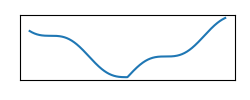
\includegraphics[width=0.4\linewidth]{./ImageFiles/Data Generation/function_example}
	\caption{Generated image example.}
	\label{fig:function_example}
\end{figure}
